\chapter*{Introduction}
\addcontentsline{toc}{chapter}{Introduction}


\chapter{Problem statement and related work}
In this chapter we introduce the reader to the problematics of genomes comparison. 
We discuss biological relevance of this problem and it's theoretical and technical challenges. 
We finis with an overview of related work.

\section{Biological motivation}

Deoxyribonucleic acid (\textbf{DNA}) is a molecule that caries genetic information of a cell, 
determining it's growth, development, functioning and reproduction. 
DNA molecules are organized in two facing strands which are composed of simpler monomer units called nucleotides.
Each nucleotide is composed of one of four nitrogen-containing nucleobases—either cytosine (C), guanine (G), adenine (A), or thymine (T).
The bases of the two separate strands are bound together according to base pairing rules (A with T, and C with G) double-stranded DNA. 

Natural representation a genome is a sequence/string of A, C, T, G corresponding to four bases. 
Note that thanks to the pairing rule we can store the genome as only the sequence for a single strand. 
The usual length of these strings is between $10^6$ and $10^10$
of characters.

It is convenient to tell a difference between multiple genome sequences. We can ask about simple characteristics like number of C bases and compare those characteristics across multiple genomes. Moreover we can ask about specific small sequences that were changed. Note figure X where we can see an absence of a sequence QW in QW genome.  

TODO real world example REDO!!!

These specific differences are called variants. 
Variants are responsible for differences. 
If we know the difference between two individuals, we can determine the variant that is responsible for this difference. 
Vice versa by detecting a variant in two genomes we, can determine otherwise undetectable difference, 
like potential start of pathogenic mutation.


\section{Genome sequencing}

Determining the genome sequence for a physical DNA is done by DNA sequencing. 
Currently most used sequencing techniques cannot read the whole sequence at once,
instead they produce set of short, overlapping substrings of sequence called reads. 
We assume that locations of these substrings are sampled uniformly across the original string.
Collection of reads for a given genome is called library.

Various read characteristics are determined by used DNA sequencing method. 
The most important ones are number of errors and length of reads.

As current sequencing techniques are rapidly improving, we did a basic overview of currently most popular ones. We only considered their attributes relevant for our problem. 
We provide overview from year $2012$ based on Quail\cite{quail2012tale} and Liu\cite{liu2012comparison}, 
as well as for $2016$ based on Goodwin \cite{goodwin2016coming}. 
The first one is important even because it is outdated, 
because we do not have date sampled with the latest methods.

\begin{table}[h]
\centering
\caption{Overview of sequence technologies for year $2012$}
\label{my-label}
\begin{tabular}{|l||l|l|l|}
Technology & Read length &   Peired reads & Cost per milion bases  \\
 &  &  &  \\
 &  &  &  \\
 &  &  & 
\end{tabular}
\end{table}



Other important form of sequencing data are paired reads. Paired reads are two reads, for which we know their approximate distance in the genome. The total reads length plus the approximated distance is referred to as insert size.


\section{Genome alignment and assembly}
One common approach to variant detection is to reconstruct the sequence based on reads and then compare reconstructed sequences. 

The sequence reconstruction problem is referred to as sequence assembly. 
Common formulation for this problem is as a shortest common superstring problem.
\begin{definicia}[Shortest common supersting] 
Given set of strings $\mathcal{P} = {S_1 , S_2 , . . . , S_k }$,
the shortest common superstring is a shortest string $S$, that contains every string from $\mathcal{P}$ as a substring. 
\end{definicia}

This problem proves to be NP-hard TODO ref (Garey and John-son, 2002).

Other common formulation is to find string by maximal likelihood. 
\begin{definicia}[Maximum likelihood supersting] 
Given set of strings $\mathcal{P} = {S_1 , S_2 , . . . , S_k }$,
the Maximum likelihood supersting is a string $S$, that maximize probability of observing $\mathcal{P}$ as a substring. 
\end{definicia}

These definitions could be extended to work with paired reads as well.

If we could reliably find the original DNA sequence, we could find variants by aligning those sequences.  TODO ref,  or more about aligning

Informally, sequence alignment is a way of arranging the sequences to identify regions of similarity. 
Aligned sequences of are typically represented as rows within a matrix. 
Gaps are inserted between the letters so that identical or similar characters are aligned in successive columns.

TODO priklad wiki  ako pekne vydno variant

Reconstructing the original sequence as defined above is often very hard.
Moreover most of the times the sequence contains a lot of errors, ambiguities and regions of low reliability. 
Sequences also contain so called repeats, which are hard to correctly assembly, but could be very important variants.

In practice there are even more problems like reverse complement, diploid genomes, errors in reads, Paired reads.
TODO CITE and REF
These can make the retrieved sequence even more ambiguous.

If we would like to know most possible variants between two sequences, we would need to have access not only to the most probable assemblies, but to all of them. This is not feasible.

\section{Problem statement}
As seen in chapter above, for the purpose of variant detection it might be better to get rid of the assembly and alignment steps. 

For this problem, some work has been already done TODO ref related work.
However proposed methods have a lot of shortcomings.
They lack concrete probabilistic foundation, do not incorporate paired reads or do not consider combinations of reads from different sources.

We would like to overcome as much of thees shortcomings and present and probabilistically 
grounded method for variant calling using paired reads and multiple sequencing technologies. 

TODO varian specification/definition. This will be added after we will see, that specific variant we can detect and describe.

\section{Related work}

\subsection{Bidirected de Bruijn graph}
A common method for representing reads is a de Bruin graph. 
This structure serves as a foundation for many assembly and alignment algorithms. TODO ref
It's mutations TODO ref are used for variant callings as well.

A de Bruijn graph TODO ref (de Bruijn and Erdos, 1946) is a structure for representing overlaps
between strings.

\begin{definicia}[de Bruijn graph]
A de Bruijn graph is directed graph. 
For given $k$, vertices of De Bruijn graph represent sequences of length $k$ ($k$-mers). 
The edges of de Bruijn graph represent possible overlaps of length $k-1$, i. e. if have have an edge $(u, v)$ and vertex $u$ represents $k$-mer $a_1 , a_2 , \cdot , a_k$ , 
then vertex $v$ represents $k$-mer $a_2 , a_3 , . . . , a_k , x$ and $k$-mer in vertex $v$ can follow $k$-mer in vertex $u$.
\end{definicia}

Intuitively an edge $(u, v)$ in de Bruijn graph represents, that $k$-mer $u$ is followed by $k$-mer $v$ in the DNA sequence.

Constructing this graph for set of reads is easy.
For each read from $ S_x \in \mathcal{P}$ we construct a set of all its $k+1$-mers. 
Each of this $k+1$-mers consist of two overlapping $k$-mers $k_1, k_2$, 
hence we can add new vertexes $k_1, k_2$ with an edge $(k_1, k_2)$ to the da Bruijn graph.
Note that each vertex can be in a graph multiple times. 
This is called coverage, and it represents the number of observations that $k_1$ if followed by $k_2$. 

De Bruijn graphs are are widely used in genome assembly and underlie many popular algorithms, including AllPaths-LG, SOAPdenovo, Abyss and Velvet. TODO refs
This approach can be extended for comparing two libraries. 
We create one de Bruijn graph out of both of them, but each vertex and each edge will be colored based on the library they are from.

If both libraries are the same, than each node and each vertex has both colors. 

\begin{definicia}[variant]
Let $a,w,w^*,b, A, B$ be strings over alphabet $\Sigma$.
Strings $a.w.b$ and $a.w^*.b$ are variants of sequences $A$ and $B$, 
if $A$ contains $a.w.b$ and $B$ contains $a.w^*.b$.
\end{definicia}

If the initial sequences $A$ and $B$ contain variants, 
those variants will show as bubbles\cite{iqbal2012novo} in the resulting de Bruijn graph.

\begin{figure}[h]
    \centering
    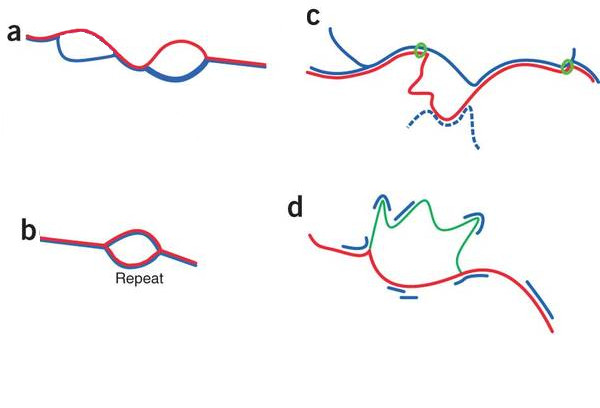
\includegraphics[width=0.5\textwidth]{images/coloreddebruijn}
    \caption{Schematic representation of methods for variation analysis using colored de Bruijn graphs. 
    Coverage is represented by line width.}
    \label{fig:mesh1}
\end{figure}


TODO draw better pictures
There is a number of ways to analyze these bubbles.
(a) The simplest $a.w.b$ and $a.w^*.b$ variant is showed as two pats that diverge and merge together forming a bubble.
(b) Repeats also form bubbles, but note that thole bubble has both colors.
(c) When the graph does not form a clean bubble, we can identify variant sites by tracking the divergence of paths.
On finding a breakpoint, we take the longest contig in the sample (that is, the path as far as the next junction) and ask whether the red path returns before this point (green circles show the anchoring sequence).
(d) The likelihood of any given genotype can be calculated from the coverage (blue) of each allele (green, red), accounting for contributions from other parts of the genome. In this example, the sample is heterozygous and therefore has coverage of both alleles, although not sufficient to enable full assembly.

Unfortunately, these approachable do not provide concrete probabilistic justification for used methods. 
Moreover they do not use information about paired reads, which proved to be valuable to decide complicated de Bruijn structures. TODO cite
 
TODO ref cite Computability of Models for Sequence Assembly

\subsection{Bubble calling}
As each variant corresponds to a bubble, we just need to find all bubbles. 

\begin{definicia}[$(s, t)$ -path]
Given two vertices $s$ and $t$ in $G$, an $(s, t)$-path is a path from $s$ to $t$. 
\end{definicia}

\begin{definicia}[$(s, t)$ -bubble]
is set of two vertex-disjoint $(s,t)$-paths. 
\end{definicia}


\begin{definicia}[$(s, t, \alpha_1, \alpha_2)$-bubble]
in a weighted directed graph is a (s, t)-bubble with paths $p_{1}$ , $p_{2}$ 
satisfying $\| p_{1} \| \leq \alpha_{1}$ and $\| p_{2} \| \leq \alpha_{2}$ .
\end{definicia}

\begin{definicia}[$(s, t, \mathcal{A})-d$-bubble] 
Let $d$ be a natural number and $A = \{\alpha_1 ,\cdot , \alpha_d \} \subset \mathcal(Q)_{\geq 0}$. 
Given a directed weighted graph $G$ and two vertices $s$ and $t$, 
a $(s, t, \mathcal{A})- d$ - bubble is a set of $d$ pairwise internally vertex-disjoint paths $\{p_1 , \cdot, p_d \}$, 
satisfying $\|p_i\| \leq \alpha_i \forall i \in [1, d]$.
\end{definicia}

For finding variants we need to solve problem of having a $(s, t, \alpha_1, \alpha_2)$-bubble.
Given a non-negatively weighted directed graph $G$, a vertex $s$,
a set $A = \{\alpha_1 ,\cdot , \alpha_d \} \subset \mathcal(Q)_{\geq 0}$ and $d \in \mathcal{N}$, decide if there exists a $(s, t, \mathcal{A})-d$-bubble in $G$ , for some $t \in V$.
This problem is a generalization of the two-disjoint-paths problem with a min-max objective function, which is NP-complete. TODO The complexity of finding two disjoint paths with min–max objective function

The same goes for problem of enumerating all bubbles in a graph.
Sacomoto et al. \cite{sacomoto2013polynomial} showed the first polynomial delay algorithm to enumerate all bubbles with length constraints in a weighted directed graph. 
Complexity of this algorithm in the best theoretical case for general graphs
is O(n(m + n log n)), hence An O(n(m + n log n)) delay algorithm. 
$n$ is the number of vertices in the graph, $m$ the number of edges. 
In the particular case of de Bruijn graphs, the complexity is $O(n(m + n log \alpha))$ where $\alpha$ is a constant related to the length of the skipped part in an alternative splicing event. 
In practice, an algorithmic solution in $O(nm log n)$ appears to work better on de Bruijn graphs built from such data. 
Sacamoto implemented the latter, and showed that it is more efficient than previous approaches and outline that it allows to discover novel long alternative splicing events.

\chapter{Proposed probabilistic approach}

TODO ideme extendovat na naozajstne DNA
TODO pridame farbu


To continue we need a few definitions. Let $v$, $w$ be two strings over alphabet $\Sigma = \{A, C, G, T \}$. Concatenation of these strings is denoted as $v . w$. 

We will extend the de Bruijn definition. TODO extended de Bruijn graph definition


\chapter{Catchy name for our tool that will be implemented.}
	\section{Probabilistic model for differences 8}
	\section{Implementation problems 8}
	\section{Used Data 3}
	\section{Results 12}
	\section{Future improvements 5}

\chapter{Evaluation}

\section{Data}
write about data generation.
\subsection{Variant simulation}
Here we closely describe methods used for variant generation, and relevant variant parameters.
\subsection{Read simulation}
Here we evaluate data for reads and we set our expectations about these data.
\subsection{Paired read simulation}
write about data sources
Here we evaluate data for paired reads and we set our expectations about these data.
\subsection{Real data}
\section{Metrics 2-3}
Here we discuss what metrics we want to improve and what is the measure of success for our solution.
\section{Benchmarks}
\subsection{Genome alignments 3-4}
Brief mentions of current genome alignments approaches.
\subsection{Without paired reads}
\subsection{Wit paired reads}


\chapter{Discussion}
Here we will discuss.



